\chapter{Planning for Overload}
\label{chap:overload}

By far, the most common cause of failure I've encountered in real-world scenarios is due to the node running out of memory. Furthermore, it is usually related to message queues going out of bounds.\footnote{Figuring out that a message queue is the problem is explained in Chapter \ref{chap:crash-dumps}, specifically in Section \ref{sec:crash-full-mailboxes}} There are plenty of ways to deal with this, but knowing which one to use will require a decent understanding of the system you're working on.

To oversimplify things, most of the projects I end up working on can be visualized as a very large bathroom sink. User and data input are flowing from the faucet. The Erlang system itself is the sink and the pipes, and wherever the output goes (whether it's a database, an external API or service, and so on) is the sewer system.

\begin{figure}[h!]
  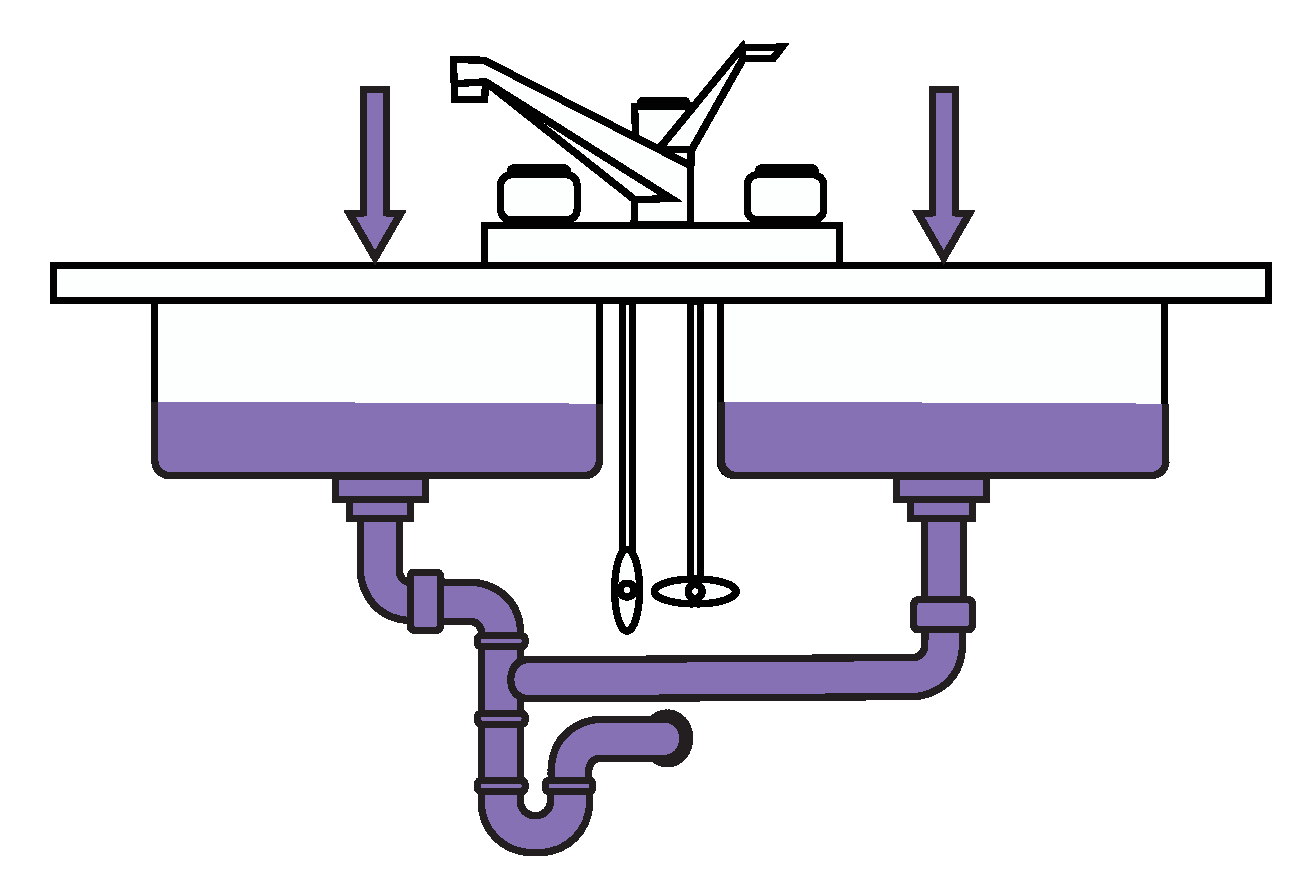
\includegraphics[max height=7cm]{sink.pdf}%
  \centering%
%  \caption{Your system is like a sink, and the true bottleneck, at the last drain, needs to be identified before you spend all your time and money making the sink and pipes bigger.}%
   \label{fig:tracing-venn}
\end{figure}

When an Erlang node dies because of a queue overflowing, figuring out who to blame is crucial. Did someone put too much water in the sink? Are the sewer systems backing up? Did you just design too small a pipe?

Determining what queue blew up is not necessarily hard. This is information that can be found in a crash dump. Finding out why it blew up is trickier. Based on the role of the process or run-time inspection, it's possible to figure out whether causes include fast flooding, blocked processes that won't process messages fast enough, and so on.

The most difficult part is to decide how to fix it. When the sink gets clogged up by too much waste, we will usually start by trying to make the bathroom sink itself larger (the part of our program that crashed, at the edge). Then we figure out the sink's drain is too small, and optimize that. Then we find out the pipes themselves are too narrow, and optimize that. The overload gets pushed further down the system, until the sewers can't take it anymore. At that point, we may try to add sinks or add bathrooms to help with the global input level.

Then there's a point where things can't be improved anymore at the bathroom's level. There are too many logs sent around, there's a bottleneck on databases that \emph{need} the consistency, or there's simply not enough knowledge or manpower in your organization to improve things there.

By finding that point, we identified what the \emph{true bottleneck} of the system was, and all the prior optimization was nice (and likely expensive), but it was more or less in vain.

We need to be more clever, and so things are moved back up a level. We try to massage the information going in the system to make it either lighter (whether it is through compression, better algorithms and data representation, caching, and so on). 

Even then, there are times where the overload will be too much, and we have to make the hard decisions between restricting the input to the system, discarding it, or accepting that the system will reduce its quality of service up to the point it will crash. These mechanisms fall into two broad strategies: back-pressure and load-shedding.

We'll explore them in this chapter, along with common events that end up causing Erlang systems to blow up.

\section{Common Overload Sources}

There are a few common causes of queues blowing up and overload in Erlang systems that most people will encounter sooner or later, no matter how they approach their system. They're usually symptomatic of having your system grow up and require some help scaling up, or of an unexpected type of failure that ends up cascading much harder than it should have.

\subsection{error\_logger Explodes}

Ironically, the process in charge of error logging is one of the most fragile ones. In a default Erlang install, the \module{error\_logger}\footnote{Defined at \href{http://www.erlang.org/doc/man/error\_logger.html}{http://www.erlang.org/doc/man/error\_logger.html}} process will take its sweet time to log things to disk or over the network, and will do so much more slowly than errors can be generated.

This is especially true of user-generated log messages (not for errors), and for crashes in large processes. For the former, this is because \module{error\_logger} doesn't really expect arbitrary levels of messages coming in continually. It's for exceptional cases only and doesn't expect lots of traffic. For the latter, it's because the entire state of processes (including their mailboxes) gets copied over to be logged. It only takes a few messages to cause memory to bubble up a lot, and if that's not enough to cause the node to run Out Of Memory (OOM), it may slow the logger enough that additional messages will.

The best solution for this at the time of writing is to use \href{https://github.com/basho/lager}{\otpapp{lager}} as a substitute logging library.

While \otpapp{lager} will not solve all your problems, it will truncate voluminous log messages, optionally drop OTP-generated error messages when they go over a certain threshold, and will automatically switch between asynchronous and synchronous modes for user-submitted messages in order to self-regulate.

It won't be able to deal with very specific cases, such as when user-submitted messages are very large in volume and all coming from one-off processes. This is, however, a much rarer occurrence than everything else, and one where the programmer tends to have more control.


\subsection{Locks and Blocking Operations}

Locking and blocking operations will often be problematic when they're taking unexpectedly long to execute in a process that's constantly receiving new tasks.

One of the most common examples I've seen is a process blocking while accepting a connection or waiting for messages with TCP sockets. During blocking operations of this kind, messages are free to pile up in the message queue.

One particularly bad example was in a pool manager for HTTP connections that I had written in a fork of the \href{https://github.com/ferd/lhttpc}{\module{lhttpc}} library. It worked fine in most test cases we had, and we even had a connection timeout set to 10 milliseconds to be sure it never took too long\footnote{10 milliseconds is very short, but was fine for collocated servers used for real-time bidding.}. After a few weeks of perfect uptime, the HTTP client pool caused an outage when one of the remote servers went down.

The reason behind this degradation was that when the remote server would go down, all of a sudden, all connecting operations would take at least 10 milliseconds, the time before which the connection attempt is given up on. With around 9,000 messages per second to the central process, each usually taking under 5 milliseconds, the impact became similar to roughly 18,000 messages a second and things got out of hand.

The solution we came up with was to leave the task of connecting to the caller process, and enforce the limits as if the manager had done it on its own. The blocking operations were now distributed to all users of the library, and even less work was required to be done by the manager, now free to accept more requests.

When there is \emph{any} point of your program that ends up being a central hub for receiving messages, lengthy tasks should be moved out of there if possible. Handling predictable overload\footnote{Something you know for a fact gets overloaded in production} situations by adding more processes — which either handle the blocking operations or instead act as a buffer while the "main" process blocks — is often a good idea.

There will be increased complexity in managing more processes for activities that aren't intrinsically concurrent, so make sure you need them before programming defensively.

Another option is to transform the blocking task into an asynchronous one. If the type of work allows it, start the long-running job and keep a token that identifies it uniquely, along with the original requester you're doing work for. When the resource is available, have it send a message back to the server with the aforementioned token. The server will eventually get the message, match the token to the requester, and answer back, without being blocked by other requests in the mean time.\footnote{The \otpapp{redo} application is an example of a library doing this, in its \href{https://github.com/heroku/redo/blob/master/src/redo\_block.erl}{redo\_block} module. The [under-documented] module turns a pipelined connection into a blocking one, but does so while maintaining pipeline aspects to the caller — this allows the caller to know that only one call failed when a timeout occurs, not all of the in-transit ones, without having the server stop accepting requests.}

This option tends to be more obscure than using many processes and can quickly devolve into callback hell, but may use fewer resources.

\subsection{Unexpected Messages}

Messages you didn't know about tend to be rather rare when using OTP applications. Because OTP behaviours pretty much expect you to handle anything with some clause in \function{handle\_info/2}, unexpected messages will not accumulate much.

However, all kinds of OTP-compliant systems end up having processes that may not implement a behaviour, or processes that go in a non-behaviour stretch where it overtakes message handling. If you're lucky enough, monitoring tools\footnote{See Section \ref{sec:global-view}} will show a constant memory increase, and inspecting for large queue sizes\footnote{See Subsection \ref{subsec:digging-procs}} will let you find which process is at fault. You can then fix the problem by handling the messages as required.

\section{Restricting Input}

Restricting input is the simplest way to manage message queue growth in Erlang systems. It's the simplest approach because it basically means you're slowing the user down (applying \emph{back-pressure}), which instantly fixes the problem without any further optimization required. On the other hand, it can lead to a really crappy experience for the user.

The most common way to restrict data input is to make calls to a process whose queue would grow in uncontrollable ways synchronously. By requiring a response before moving on to the next request, you will generally ensure that the direct source of the problem will be slowed down.

The difficult part for this approach is that the bottleneck causing the queue to grow is usually not at the edge of the system, but deep inside it, which you find after optimizing nearly everything that came before. Such bottlenecks will often be database operations, disk operations, or some service over the network. 

This means that when you introduce synchronous behaviour deep in the system, you'll possibly need to handle back-pressure, level by level, until you end up at the system's edges and can tell the user, "please slow down."
Developers that see this pattern will often try to put API limits per user\footnote{There's a tradeoff between slowing down all requests equally or using rate-limiting, both of which are valid. Rate-limiting per user would mean you'd still need to increase capacity or lower the limits of all users when more new users hammer your system, whereas a synchronous system that indiscriminately blocks should adapt to any load with more ease, but possibly unfairly.} on the system entry points. This is a valid approach, especially since it can guarantee a basic quality of service (QoS) to the system and allows one to allocate resources as fairly (or unfairly) as desired.
  
\subsection{How Long Should a Time Out Be}

What's particularly tricky about applying back-pressure to handle overload via synchronous calls is having to determine what the typical operation should be taking in terms of time, or rather, at what point the system should time out.

The best way to express the problem is that the first timer to be started will be at the edge of the system, but the critical operations will be happening deep within it. This means that the timer at the edge of the system will need to have a longer wait time that those within, unless you plan on having operations reported as timing out at the edge even though they succeeded internally. 

An easy way out of this is to go for infinite timeouts. Pat Helland\footnote{\href{http://queue.acm.org/detail.cfm?id=2187821}{Idempotence is Not a Medical Condition}, April 14, 2012} has an interesting answer to this:

\begin{quote}
Some application developers may push for no timeout and argue it is OK to wait indefinitely. I typically propose they set the timeout to 30 years. That, in turn, generates a response that I need to be reasonable and not silly. \emph{Why is 30 years silly but infinity is reasonable?} I have yet to see a messaging application that really wants to wait for an unbounded period of time…
\end{quote}

This is, ultimately, a case-by-case issue. In many cases, it may be more practical to use a different mechanism for that flow control.\footnote{In Erlang, using the value \term{infinity} will avoid creating a timer, avoiding some resources. If you do use this, remember to at least have a well-defined timeout somewhere in the sequence of calls.}

\subsection{Asking For Permission}

A somewhat simpler approach to back-pressure is to identify the resources we want to block on, those that cannot be made faster and are critical to your business and users. Lock these resources behind a module or procedure where a caller must ask for the right to make a request and use them. There's plenty of variables that can be used: memory, CPU, overall load, a bounded number of calls, concurrency, response times, a combination of them, and so on.

The \emph{SafetyValve}\footnote{\href{https://github.com/jlouis/safetyvalve}{https://github.com/jlouis/safetyvalve}} application is a system-wide framework that can be used when you know back-pressure is what you'll need.

For more specific use cases having to do with service or system failures, there are plenty of circuit breaker applications available. Examples include \otpapp{breaky}\footnote{\href{https://github.com/mmzeeman/breaky}{https://github.com/mmzeeman/breaky}}, \otpapp{fuse}\footnote{\href{https://github.com/jlouis/fuse}{https://github.com/jlouis/fuse}},  or Klarna's \otpapp{circuit\_breaker}\footnote{\href{https://github.com/klarna/circuit\_breaker}{https://github.com/klarna/circuit\_breaker}}.

Otherwise, ad-hoc solutions can be written using processes, ETS, or any other tool available. The important part is that the edge of the system (or subsystem) may block and ask for the right to process data, but the critical bottleneck in code is the one to determine whether that right can be granted or not.

The advantage of proceeding that way is that you may just avoid all the tricky stuff about timers and making every single layer of abstraction synchronous. You'll instead put guards at the bottleneck and at a given edge or control point, and everything in between can be expressed in the most readable way possible.

\subsection{What Users See}

The tricky part about back-pressure is reporting it. When back-pressure is done implicitly through synchronous calls, the only way to know it is at work due to overload is that the system becomes slower and less usable. Sadly, this is also going to be a potential symptom of bad hardware, bad network, unrelated overload, and possibly a slow client.

Trying to figure out that a system is applying back-pressure by measuring its responsiveness is equivalent to trying to diagnose which illness someone has by observing that person has a fever. It tells you something is wrong, but not what.

Asking for permission, as a mechanism, will generally allow you to define your interface in such a way that you can explicitly report what is going on: the system as a whole is overloaded, or you're hitting a limit into the rate at which you can perform an operation and adjust accordingly.

There is a choice to be made when designing the system. Are your users going to have per-account limits, or are the limits going to be global to the system?

System-global or node-global limits are usually easy to implement, but will have the downside that they may be unfair. A user doing 90\% of all your requests may end up making the platform unusable for the vast majority of the other users.

Per-account limits, on the other hand, tend to be very fair, and allow fancy schemes such as having premium users who can go above the usual limits. This is extremely nice, but has the downside that the more users use your system, the higher the effective global system limit tends to move. Starting with 100 users that can do 100 requests a minute gives you a global 10000 requests per minute. Add 20 new users with that same rate allowed, and suddenly you may crash a lot more often.

The safe margin of error you established when designing the system slowly erodes as more people use it. It's important to consider the tradeoffs your business can tolerate from that point of view, because users will tend not to appreciate seeing their allowed usage go down all the time, possibly even more so than seeing the system go down entirely from time to time.


\section{Discarding Data}

When nothing can slow down outside of your Erlang system and things can't be scaled up, you must either drop data or crash (which drops data that was in flight, for most cases, but with more violence).

It's a sad reality that nobody really wants to deal with. Programmers, software engineers, and computer scientists are trained to purge the useless data, and keep everything that's useful. Success comes through optimization, not giving up.

However, there's a point that can be reached where the data that comes in does so at a rate faster than it goes out, even if the Erlang system on its own is able to do everything fast enough. In some cases, It's the component \emph{after} it that blocks.

If you don't have the option of limiting how much data you receive, you then have to drop messages to avoid crashing.

\subsection{Random Drop}

Randomly dropping messages is the easiest way to do such a thing, and might also be the most robust implementation, due to its simplicity.

The trick is to define some threshold value between 0.0 and 1.0 and to fetch a random number in that range:

\includecode[erlang]{drop.erl}

If you aim to keep 95\% of the messages you send, the authorization could be written by a call to \expression{case drop:random(0.95) of true -> send(); false -> drop() end}, or a shorter \expression{drop:random(0.95) andalso send()} if you don't need to do anything specific when dropping a message. 

The \function{maybe\_seed()} function will check that a valid seed is present in the process dictionary and use it rather than a crappy one, but only if it has not been defined before, in order to avoid calling \function{now()} (a monotonic function that requires a global lock) too often.

There is one `gotcha' to this method, though: the random drop must ideally be done at the producer level rather than at the queue (the receiver) level. The best way to avoid overloading a queue is to not send data its way in the first place. Because there are no bounded mailboxes in Erlang, dropping in the receiving process only guarantees that this process will be spinning wildly, trying to get rid of messages, and fighting the schedulers to do actual work.

On the other hand, dropping at the producer level is guaranteed to distribute the work equally across all processes.

This can give place to interesting optimizations where the working process or a given monitor process\footnote{Any process tasked with checking the load of specific processes using heuristics such as \expression{process\_info(Pid, message\_queue\_len)} could be a monitor} uses values in an ETS table or \function{application:set\_env/3} to dynamically increase and decrease the threshold to be used with the random number. This allows control over how many messages are dropped based on overload, and the configuration data can be fetched by any process rather efficiently by using \function{application:get\_env/2}.

Similar techniques could also be used to implement different drop ratios for different message priorities, rather than trying to sort it all out at the consumer level.

\subsection{Queue Buffers}

Queue buffers are a good alternative when you want more control over the messages you get rid of than with random drops, particularly when you expect overload to be coming in bursts rather than a constant stream in need of thinning.

Even though the regular mailbox for a process has the form of a queue, you'll generally want to pull \emph{all} the messages out of it as soon as possible. A queue buffer will need two processes to be safe:

\begin{itemize*}
	\item The regular process you'd work with (likely a \module{gen\_server});
	\item A new process that will do nothing but buffer the messages. Messages from the outside should go to this process.
\end{itemize*}

To make things work, the buffer process only has to remove all the messages it can from its mail box and put them in a queue data structure\footnote{The \module{queue} module in Erlang provides a purely functional queue data structure that can work fine for such a buffer.} it manages on its own. Whenever the server is ready to do more work, it can ask the buffer process to send it a given number of messages that it can work on. The buffer process picks them from its queue, forwards them to the server, and goes back to accumulating data.

Whenever the queue grows beyond a certain size\footnote{To calculate the length of a queue, it is preferable to use a counter that gets incremented and decremented on each message sent or received, rather than iterating over the queue every time. It takes slightly more memory, but will tend to distribute the load of counting more evenly, helping predictability and avoiding more sudden build-ups in the buffer's mailbox} and you receive a new message, you can then pop the oldest one and push the new one in there, dropping the oldest elements as you go.\footnote{You can alternatively make a queue that pops the newest message and queues up the oldest ones if you feel previous data is more important to keep.}

This should keep the entire number of messages received to a rather stable size and provide a good amount of resistance to overload, somewhat similar to the functional version of a ring buffer.

The \emph{PO Box}\footnote{Available at: \href{https://github.com/ferd/pobox}{https://github.com/ferd/pobox}, the library has been used in production for a long time in large scale products at Heroku and is considered mature} library implements such a queue buffer.

\subsection{Stack Buffers}

Stack buffers are ideal when you want the amount of control offered by queue buffers, but you have an important requirement for low latency.

To use a stack as a buffer, you'll need two processes, just like you would with queue buffers, but a list\footnote{Erlang lists \emph{are} stacks, for all we care. They provide push and pop operations that take O(1) complexity and are very fast} will be used instead of a queue data structure.

The reason the stack buffer is particularly good for low latency is related to issues similar to bufferbloat\footnote{\href{http://queue.acm.org/detail.cfm?id=2071893}{http://queue.acm.org/detail.cfm?id=2071893 }}. If you get behind on a few messages being buffered in a queue, all the messages in the queue get to be slowed down and acquire milliseconds of wait time. Eventually, they all get to be too old and the entire buffer needs to be discarded.

%% Image of queue taking long from RTB article. Maybe side image or side explanation?

On the other hand, a stack will make it so only a restricted number of elements are kept waiting while the newer ones keep making it to the server to be processed in a timely manner.

%% image of queue taking a short time from RTB article.

Whenever you see the stack grow beyond a certain size or notice that an element in it is too old for your QoS requirements you can just drop the rest of the stack and keep going from there. \emph{PO Box} also offers such a buffer implementation.

A major downside of stack buffers is that messages are not necessarily going to be processed in the order they were submitted — they're nicer for independent tasks, but will ruin your day if you expect a sequence of events to be respected.

\subsection{Time-Sensitive Buffers}

If you need to react to old events \emph{before} they are too old, then things become more complex, as you can't know about it without looking deep in the stack each time, and dropping from the bottom of the stack in a constant manner gets to be inefficient. An interesting approach could be done with buckets, where multiple stacks are used, with each of them containing a given time slice. When requests get too old for the QoS constraints, drop an entire bucket, but not the entire buffer.

It may sound counter-intuitive to make some requests a lot worse to benefit the majority — you'll have great medians but poor 99 percentiles — but this happens in a state where you would drop messages anyway, and is preferable in cases where you do need low latency.

\subsection{Dealing With Constant Overload}

Being under constant overload may require a new solution. Whereas both queues and buffers will be great for cases where overload happens from time to time (even if it's a rather prolonged period of time), they both work more reliably when you expect the input rate to eventually drop, letting you catch up.

You'll mostly get problems when trying to send so many messages they can't make it all to one process without overloading it. Two approaches are generally good for this case:

\begin{itemize*}
	\item Have many processes that act as buffers and load-balance through them (scale horizontally)
	\item use ETS tables as locks and counters (reduce the input)
\end{itemize*}

ETS tables are generally able to handle a ton more requests per second than a process, but the operations they support are a lot more basic. A single read, or adding or removing from a counter atomically is as fancy as you should expect things to get for the general case.

ETS tables will be required for both approaches.

Generally speaking, the first approach could work well with the regular process registry: you take \var{N} processes to divide up the load, give them all a known name, and pick one of them to send the message to. Given you're pretty much going to assume you'll be overloaded, randomly picking a process with an even distribution tends to be reliable: no state communication is required, work will be shared in a roughly equal manner, and it's rather insensitive to failure.

In practice, though, we want to avoid atoms generated dynamically, so I tend to prefer to register workers in an ETS table with \expression{read\_concurrency} set to \expression{true}. It's a bit more work, but it gives more flexibility when it comes to updating the number of workers later on.

An approach similar to this one is used in the \module{lhttpc}\footnote{The \href{https://github.com/ferd/lhttpc/blob/master/src/lhttpc\_lb.erl}{lhttpc\_lb} module in this library implements it.} library mentioned earlier, to split load balancers on a per-domain basis.

For the second approach, using counters and locks, the same basic structure still remains (pick one of many options, send it a message), but before actually sending a message, you must atomically update an ETS counter\footnote{By using \function{ets:update\_counter/3}.}. There is a known limit shared across all clients (either through their supervisor, or any other config or ETS value) and each request that can be made to a process needs to clear this limit first.

This approach has been used in \module{dispcount}\footnote{\href{https://github.com/ferd/dispcount}{https://github.com/ferd/dispcount}} to avoid message queues, and to guarantee low-latency responses to any message that won't be handled so that you do not need to wait to know your request was denied. It is then up to the user of the library whether to give up as soon as possible, or to keep retrying with different workers.

\subsection{How Do You Drop}

Most of the solutions outlined here work based on message quantity, but it's also possible to try and do it based on message size, or expected complexity, if you can predict it. When using a queue or stack buffer, instead of counting entries, all you may need to do is count their size or assign them a given load as a limit.

I've found that in practice, dropping without regard to the specifics of the message works rather well, but each application has its share of unique compromises that can be acceptable or not\footnote{Old papers such as \href{http://research.microsoft.com/en-us/um/people/blampson/33-hints/webpage.html}{Hints for Computer System Designs} by Butler W. Lampson recommend dropping messages: "Shed load to control demand, rather than allowing the system to become overloaded." The paper also mentions that  "A system cannot be expected to function well if the demand for any resource exceeds two-thirds of the capacity, unless the load can be characterized extremely well." adding that "The only systems in which cleverness has worked are those with very well-known loads."}.

There are also cases where the data is sent to you in a "fire and forget" manner — the entire system is part of an asynchronous pipeline — and it proves difficult to provide feedback to the end-user about why some requests were dropped or are missing. If you can reserve a special type of message that accumulates dropped responses and tells the user "\var{N} messages were dropped for reason \var{X}", that can, on its own, make the compromise far more acceptable to the user. This is the choice that was made with Heroku's \href{https://devcenter.heroku.com/articles/logplex}{logplex} log routing system, which can spit out \href{https://devcenter.heroku.com/articles/error-codes\#l10-drain-buffer-overflow}{L10 errors}, alerting the user that a part of the system can't deal with all the volume right now.

In the end, what is acceptable or not to deal with overload tends to depend on the humans that use the system. It is often easier to bend the requirements a bit than develop new technology, but sometimes it is just not avoidable.


\section{Exercises}

\subsection*{Review Questions}

\begin{enumerate}
	\item Name the common sources of overload in Erlang systems
	\item What are the two main classes of strategies to handle overload?
	\item How can long-running operations be made safer?
	\item When going synchronous, how should timeouts be chosen?
	\item What is an alternative to having timeouts?
	\item When would you pick a queue buffer before a stack buffer?
\end{enumerate}

\subsection*{Open-ended Questions}

\begin{enumerate}
	\item What is a \emph{true bottleneck}? How can you find it?
	\item In an application that calls a third party API, response times vary by a lot depending on how healthy the other servers are. How could one design the system to prevent occasionally slow requests from blocking other concurrent calls to the same service?
	\item What's likely to happen to new requests to an overloaded latency-sensitive service where data has backed up in a stack buffer? What about old requests?
	\item Explain how you could turn a load-shedding overload mechanism into one that can also provide back-pressure.
	\item Explain how you could turn a back-pressure mechanism into a load-shedding mechanism. 
	\item What are the risks, for a user, when dropping or blocking a request? How can we prevent duplicate messages or missed ones?
	\item What can you expect to happen to your API design if you forget to deal with overload, and suddenly need to add back-pressure or load-shedding to it?
\end{enumerate}


%%% Cognitive
%%
%% Knowledge: recall facts, terms, basic concepts
%% 
%% - Name the common sources of overload in Erlang systems
%% - What are the two main classes of strategies to handle overload?
%%
%% Comprehension: organizing, comparing, translating, interpreting, giving descriptions, and stating the main ideas
%%
%% - Why is it that error_logger may cause failures? How can they be fixed?
%% - When can long-running operations become problematic?
%% - How can long-running operations be made safer?
%% - When going synchronous, how should timeouts be chosen?
%% - What is an alternative to having timeouts?
%% - What are ways to communicate overload to users?
%% - What can you do when you can't slow down data input?
%% - Is there a different approach to be taken between temporary and permanent overload?
%%
%% Application: Solve problems in new situations by applying acquired knowledge, facts, techniques and rules in a different way
%%
%% - How can you find what is a 'true bottleneck' ?
%% - In an application that calls a third party API, response times vary by a lot depending on how healthy the other servers are. How could one design the system to prevent occasionally slow requests from blocking other ones?
%% - When would you pick a queue buffer before a stack buffer? 
%% - Which end should you drop items from in a queue buffer, and when?
%%
%% Analysis: break down info, make inferences, find evidence
%% - What's likely to happen to new requests to an overloaded latency-sensitive service where data has backed up in a stack buffer? What about old ones?
%% - What can you expect about response times if an app is permanently overloaded while using a queue buffer?
%% - 
%%
%% Synthesis: Compile information together in a different way by combining elements in a new pattern or proposing alternative solutions
%%
%% - Explain how you could turn a lossy overload mechanism ( into one that can also provide back-pressure.
%% - Explain how you could turn a back-pressure mechanism into a lossy overload 
%% - Can you think of application designs where lager can't save you of error_logger issues?
%%
%% Evaluation: Present and defend opinions by making judgments about information
%%
%% - What are the risks, for a user, when dropping or blocking a request? How can we prevent duplicate submissions or missed ones?
%% - Which form of overload management would be most appropriate for a bank? For an online polling system?
%% - What can you expect to happen to your API design if you forget to deal with overload, and suddenly need to add back-pressure or load-shedding to it?
%% - What positive points could you think of when using infinite timeouts?


%%%
%%%
%%%

